\chapter{Literature Review}
\label{chapter:literature}

% #TODO Overview of literature review section


\section{Visual Question Answering Metrics}

In their seminal VQA paper, \citeauthor{malinowski2014multiworld} \cite{malinowski2014multiworld} note that traditional accuracy measures fail to capture partial correctness of answers; given a ground-truth answer `carton', the traditional accuracy metric would give zero weight to the answer `box', despite the semantic similarity between the ground-truth and predicted answers. In general, larger answer vocabularies typically lead to blurrier semantic boundaries between answer classes when compared to datasets with a smaller answer vocabulary like CIFAR \cite{krizhevsky2009learning}. Since datasets that frame the VQA problem as a classification task typically have a large answer vocabulary containing objects, numbers, colours and other concepts, it follows that an effective VQA metric should reward answers that are partially correct or share semantics with the ground-truth answer.

Metric design becomes even more important when considering full-sentence answers instead of single-word answers; evaluation of full-sentence answers requires metrics that are robust under semantic and syntactic variations between predicted and ground truth answers. A variety of natural language generation (NLG) metrics \cite{papineni2002bleu, lin2004rouge, banerjee2005meteor, vedantam2015cider} have been applied to image captioning tasks \cite{chen2015microsoft}, and are consequently applicable to open-ended VQA. Unfortunately, each of these metrics have their own advantages and pitfalls, so multiple metrics need to be considered to gain useful insights into model performance.

% Although I focus on VQA as a multi-class classification problem in this dissertation, I provide a brief overview of these metrics in section \ref{subsection:open_ended_vqa_metrics}.

In the following subsections, I explore a variety of metrics for both class-based and free-form VQA tasks as outlined in Table \ref{tab:vqa_metrics_suitability}, focusing on how they reward partially correct answers.


\begin{table}[htbp]
    \centering
    \begin{xltabular}{\linewidth}{@{}lCCCl@{}}
        \toprule
        \multicolumn{1}{c}{\multirow{2}{*}{\textbf{Metric}}} & \multicolumn{3}{c}{\textbf{Suitability}}                                                           & \multicolumn{1}{c}{\multirow{2}{*}{\textbf{Common Uses}}} \\ \cmidrule(lr){2-4}
        \multicolumn{1}{c}{}                                 & \multicolumn{1}{c}{Multi-class} & \multicolumn{1}{c}{Multi-label} & \multicolumn{1}{c}{Open-ended} & \multicolumn{1}{c}{}                                      \\ \midrule
        Accuracy                                             & \checkmark                      & \checkmark                      &                                & Multiple                                                  \\
        WUPS                                                 & \checkmark                      & \checkmark                      &                                & Multiple                                                  \\
        Consensus Accuracy                                   & \checkmark                      & \checkmark                      &                                & VQA                                                       \\
        Consistency                                          & \checkmark                      & \checkmark                      &                                & VQA                                                       \\
        Validity                                             & \checkmark                      &                                 &                                & VQA                                                       \\
        Plausibility                                         & \checkmark                      &                                 &                                & VQA                                                       \\
        Grounding                                            & \checkmark                      & \checkmark                      & \checkmark                     & VQA                                                       \\
        Distribution                                         & \checkmark                      &                                 &                                & VQA                                                       \\
        BLEU                                                 &                                 &                                 & \checkmark                     & Machine translation                                       \\
        ROUGE                                                &                                 &                                 & \checkmark                     & Text summarisation                                        \\
        METEOR                                               &                                 &                                 & \checkmark                     & Machine translation                                       \\
        CIDEr                                                &                                 &                                 & \checkmark                     & Image captioning                                          \\ \bottomrule
        \caption[Suitability of metrics for various VQA tasks]{A comparison of metrics and their suitability for various VQA tasks.}
        \label{tab:vqa_metrics_suitability}
    \end{xltabular}
\end{table}

\begin{table}[htbp]
    \begin{footnotesize}
      \begin{xltabular}{\linewidth}{@{}lLL@{}}
        \toprule
            \multicolumn{1}{c}{\textbf{Metric}} & \multicolumn{1}{c}{\textbf{Advantages}}                                                    & \multicolumn{1}{c}{\textbf{Disadvantages}}                                                                                                                              \\ \midrule
            Accuracy                            & - Simple and interpretable.                                                                & - Penalises slightly incorrect answers harshly.                                                                                                                         \\
                                                & - Suitable for problems with a small answer set cardinality.                               & - Requires an exact set of answers for multi-label tasks.                                                                                                               \\ \midrule
            WUPS                                & - Rewards incorrect but semantically similar answers.                                      & - Rewards answers that share a concept class \textit{e.g.} \textit{`colour'} with the true answer but have opposite meanings e.g. \textit{`white'} vs \textit{`black'}. \\
                                                &                                                                                            & - Evaluating open-ended answers ignores sentence syntax and context.                                                                                                    \\ \midrule
            Consensus Accuracy                  & - Simple and interpretable.                                                                & - Multiple correct reference answers may be contradictory.                                                                                                              \\
                                                & - Aligns with human answers.                                                               & - Not all questions have 3 matching reference answers                                                                                                                   \\
                                                &                                                                                            & - Reference answers are expensive to collect.                                                                                                                           \\ \midrule
            Consistency                         & - Ensures models avoid contradictory answers to related questions.                         & - Requires a set of entailed questions for each question.                                                                                                               \\
                                                &                                                                                            & - Limited by the usefulness of the accuracy metric                                                                                                                      \\ \midrule
            Validity                            & - Measures a model's ability to respond to various question types.                         & - Requires a set of valid answers for each question type.                                                                                                               \\ \midrule
            Plausibility                        & - Ensures models avoid nonsensical answers.                                                & - Requires scene graphs for all dataset samples.                                                                                                                        \\
                                                &                                                                                            & - Can be imprecise for sparsely occurring objects.                                                                                                                      \\ \midrule
            Grounding                           & - Ensures models use image data to answer questions instead of exploiting language priors. & - Only applicable to attention-based models.                                                                                                                            \\
                                                &                                                                                            & - Requires knowledge about which image regions are relevant to each dataset sample.                                                                                     \\ \midrule
            Distribution                        & - Ensures models respond well to all question subject-type groups                          &                                                                                                                                                                         \\ \midrule
            BLEU                                & - \(n\)-grams capture positional relationships between words.                              & - Requires multiple ground truth answers for good performance.                                                                                                          \\
                                                & - Penalises answers that are too short or too long.                                        & - Performs better for entire corpora compared to individual sentences due to the corpus-level brevity penalty, an issue for VQA.                                        \\
                                                &                                                                                            & - A zero score for any \(n\)-gram component gives a zero BLEU score.                                                                                                    \\ \midrule
            ROUGE                               & - \(n\)-grams capture positional relationships between words.                              &                                                                                                                                                                         \\ \midrule
            METEOR                              & - Accounts for synonyms                                                                    &                                                                                                                                                                         \\
                                                & - Accounts for morphological discrepancies                                                 &                                                                                                                                                                         \\
                                                & - Accounts for both precision and recall                                                   &                                                                                                                                                                         \\ \bottomrule
    \caption[Advantages and disadvantages of metrics for various VQA tasks]{A comparison of metrics and their advantages and disadvantages for various VQA tasks.}
    \label{tab:vqa_metrics_comparison}
    \end{xltabular}
  \end{footnotesize}
\end{table}

\subsection{Semantic Similarity Measures}

\subsubsection{Wu-Palmer Similarity}

Originally coined the ``conceptual similarity measure'' \cite{wu1994verbs}, the now-labelled Wu-Palmer (WUP) similarity is used to measure the semantic similarity of two concepts based on their positions in a taxonomy tree such as WordNet \cite{miller1995wordnet}. Formally, given two concepts \(A\) and \(B\) in a taxonomy tree \(T\), we define the Wu-Palmer similarity of \(A\) and \(B\) as

\begin{equation}
    WUP(A, B) = \frac{2 N_C}{N_A + N_B + 2 N_C}
    \label{eq:wup}
\end{equation}

where \(N_A\) and \(N_B\) are the number of edges from \(A\) and \(B\) to their lowest common ancestor \(C\) respectively, and \(N_C\) is the depth of \(C\) in \(T\), as illustrated in Figure \ref{fig:wups_tree}.

\begin{figure}[H]
    \centering
    \begin{forest}
      [ROOT [C, edge=dashed, edge label={node[midway,auto]{\(N_C\)}} [A, edge=dashed, edge label={node[midway,left]{\(N_A\)}}] [B, edge=dashed, edge label={node[midway,right]{\(N_B\)}}]]]
    \end{forest}
    \caption[A taxonomy tree describing the relationship between two concepts.]{Given two concepts \(A\) and \(B\), \(C\) denotes the ``least common superconcept'' of A and B. (Figure adapted from \cite{wu1994verbs})}
    \label{fig:wups_tree}
\end{figure}

Given this definition, it naturally follows that two equal concepts occupy the same position in the taxonomy tree and thus have a similarity of 1, whilst two concepts whose lowest common ancestor is the root of the tree have a similarity of 0.

Whilst WUP similarity can capture similarities between a target and predicted concept, \citeauthor{malinowski2014multiworld} extend WUP similarity to sets of concepts, proposing the WUP set score for evaluation of multi-label classification tasks:

\begin{equation}
    \textsc{WUPS}(A, B) = \frac{1}{N} \sum_{i=1}^N \min \{\prod_{a \in A_i} \max_{b \in B_i} \textsc{WUP}(a, b), \prod_{b \in B_i} \max_{a \in A_i} \textsc{WUP}(a, b)\}
    \label{eq:wups}
\end{equation}

To apply this metric to VQA tasks, we let \(A\) and \(B\) be a sequence of sets of predicted and ground-truth answers respectively, each of size \(N\). Noting that \(WUP(A_i, B_i) \in [0, 1]\) for each \(A_i \in A\) and \(B_i \in B\), the following useful properties of the metric become evident:

\begin{enumerate}
    \item \(WUPS(A, B) \in [0, 1]\), with \(WUPS(A, B) = 1\) when \(A = B\).
    \item Naive models which overestimate the number of target answers will be penalised according to how dissimilar the additional provided answers are to their closest target answer.
    \item Models which underestimate the number of target answers \textit{i.e.} \(|A_i| < |B_i|\) will be penalised, with a harsher penalty if the concepts in the target set are dissimilar.
\end{enumerate}

The authors note that WUP yields large values for related but not interchangeable concepts, noting that \(WUP(\text{carton}, \text{box}) = 0.94\) where \(WUP(\text{stove}, \text{fire extinguisher}) = 0.82\). To encourage precise answers and avoid accepting related but inaccurate answers, the authors down-weight \(WUP(a, b)\) by a ratio \(r = 0.1\) whenever it is less than some threshold \(t = 0.9\).

While this down-weighting alleviates this issue for questions that query objects in an image, answers to questions about object attributes and colours are often poorly evaluated; \citeauthor{kafle2017visual} note that even after down-weighting \(WUP\) scores, \(WUPS(\text{white}, \text{black}) = 0.91\). Whilst the metric correctly rewards the answerer for correctly identifying that the answer to the question is a colour, a score of 0.91 seems too high, highlighting the non-linearity of the metric that makes it more difficult to interpret at a glance unlike other common metrics like accuracy.

By nature, the metric also operates on single WordNet concepts, which often coincide with single words. To evaluate full-sentence or even multi-word answers with WUPS, we must treat sentences as a set of distinct words, disregarding essential syntactic and contextual information. This makes WUPS a poor candidate for open-ended VQA evaluation when compared to other NLG metrics such as BLEU, ROUGE, METEOR and CIDEr, as briefly discussed in section \ref{subsection:open_ended_vqa_metrics} and summarised in table \ref{tab:vqa_metrics_comparison}.

%In addition to this issue, the down-weighting approach introduces two new parameters which increase the complexity and subjectivity of the metric. 


% \[
% \min \{\prod_{a \in A_i} \max_{b \in B_i} WUP(a, b), \prod_{b \in B_i} \max_{a \in A_i} WUP(a, b)\} =  \begin{cases}
%     1, &\text{if } A_i = B_i \\
%     \prod_{b \in B_i} \max_{a \in A_i} WUP(a, b) < 1, &\text{if } A_i \subset B_i \\
%     \prod_{a \in A_i} \max_{b \in B_i} WUP(a, b) < 1, &\text{if } A_i \supset B_i
% \end{cases}
% \]

\subsection{Consensus Measures}
\label{subsection:consensus_measures}

\subsubsection{VQA Consensus Accuracy}
Introduced by \citeauthor{antol2015vqa} in \citeyear{antol2015vqa}, the VQA consensus accuracy metric is the most common metric used to benchmark VQA models, due to the widespread adoption of the VQA dataset and its variants. To reward partially correct answers, VQA consensus accuracy compares a candidate answer to multiple reference answers, provided by humans via crowdsourcing platforms like Amazon Mechanical Turk (AMT) in the case of the VQA dataset. The VQA consensus accuracy metric is defined as

\begin{equation}
    \textsc{Accuracy} = \min \left( \frac{n}{3}, 1 \right)
    \label{eq:vqa_consensus_accuracy}
\end{equation}

where \(n\) is the number of answers in the set of reference answers that match a given candidate answer, \textit{i.e.} an answer is considered entirely correct if it matches 3 or more of the 10 reference answers for the corresponding question and image.

At a surface level, the metric is interpretable and can reward multiple correct and/or partially correct answers effectively, however, the latter can become a disadvantage depending on the quality of the reference answers. In their analysis of the VQAv1 dataset, \citeauthor{kafle2017visual} point out that 16.7\% of questions have less than 3 matching answers in their group of 10 reference answers, capping the performance of a perfect VQA model. A large contributor to this statistic is the presence of multi-word answers in the dataset; 89.32\% of answers in the VQAv1 dataset are single-word answers, leaving ample room for disagreement amongst reference answers.

Moreover, supporting multiple correct answers is unfavourable if the correct answers are contradictory. Again, \citeauthor{kafle2017visual} identify that 13\% of VQA v1 yes/no questions contain both `yes' and `no' 3 or more times in their group of 10 reference answers, making both options entirely correct.


% \begin{itemize}
%     \item ``Inter-human agreement is only 83.3\%. It is impossible for an algorithm to achieve 100\% accuracy.''\cite{kafle2017visual} % no consensus answer problem
%     \item even when counting only those answers in the VQAv2 training set that appear more than 8 times, there are still 3129 unique reference answers. After this selection,  \cite{teney2018tips}.
% \end{itemize}

\subsubsection{DAQUAR Consensus Measures}

Motivated by the relatively poor human baseline performance (Accuracy: 50.20\%, WUPS@0.9:  50.82\%) on the DAQUAR dataset, \citeauthor{malinowski2015ask} extended the dataset by collecting an average of 5 reference answers for each image-question pair and developing two consensus metrics based on their previous WUPS measure:

\begin{equation}
    \textsc{WUPS}_{\text{mean}}(A, B) =     \frac{1}{NK} \sum_{i=1}^N \sum_{i=1}^K \min \{\prod_{a \in A_i} \max_{b \in B_i} \textsc{WUP}(a, b), \prod_{b \in B_i} \max_{a \in A_i} \textsc{WUP}(a, b)\}
    \label{eq:wups_mean_consensus}
\end{equation}


\begin{equation}
    \textsc{WUPS}_{\text{min}}(A, B) =     \frac{1}{N} \sum_{i=1}^N \max_{k=1}^K \left( \min \{\prod_{a \in A_i} \max_{b \in B_i} \textsc{WUP}(a, b), \prod_{b \in B_i} \max_{a \in A_i} \textsc{WUP}(a, b)\} \right)
    \label{eq:wups_min_consensus}
\end{equation}

where \(N\), \(A\) and \(B\) are as defined in Equation \ref{eq:wups}, and \(K\) is the number of reference answers for the \(i\)-th dataset sample.

The mean consensus metric rewards candidate answers that coincide with more frequent reference answers, whilst the minimum consensus metric rewards candidate answers according to their similarity to the closest reference answer.

\subsection{GQA Metrics}
\subsubsection{Consistency}
\subsubsection{Validity}
\subsubsection{Plausibility}
\subsubsection{Grounding}
\subsubsection{Distribution}

\subsection{Metrics for Open-ended VQA}
\label{subsection:open_ended_vqa_metrics}

Given the challenge of multi-class and multi-label VQA tasks, there has been little research into open-ended VQA task, even though some datasets contain full-sentence answers for each question. In addition, research into open-ended VQA has been stunted by the lack of a widely accepted metric for the task; metrics such as BLEU,  ROUGE, METEOR and CIDEr were originally developed for other tasks as shown in Table \ref{tab:vqa_metrics_comparison}, and thus have various disadvantages when used in VQA contexts.

BLEU and METEOR were originally developed for automatic evaluation of machine translation systems.

{\color{red} require multiple reference translations for good functionality \(\rightarrow\) Missing from VQA datasets}

\subsubsection{BLEU}

\textbf{Motivations:}

\begin{itemize}
    \item Machine translation
    \item Human evaluation can take months
    \item Bi-Lingual Evaluation Understudy (BLEU) is:
    \begin{itemize}
        \item ``Quick''
        \item ``Inexpensive''
        \item ``Language independent''
        \item Accurate (``Correlates highly with human evaluation'')
    \end{itemize}
    \item Created in an effort to reduce the evaluation bottleneck on machine translation progress and promote more rapid prototyping of ideas.
    \item Derived from word-error-rate metric used in speech recognition, modified to allow for subtle word reorderings and substitutions.
\end{itemize}


\textbf{General Caveats:}

\begin{itemize}
    \item Relies on multiple ground truth sentences with different flavours/styles (translations for NMT, answers for VQA or image captioning). BLEU does better on a large corpus than for individual sentences.
    \item Performs better for entire corpora compared to individual sentences due to the corpus-level brevity penalty.
    \item Brevity penalty is required to avoid short answers like ``of the'', where there is only one \(2\)-gram which is likely to occur in ground truth answers but contains no useful contextual information.
\end{itemize}


\textbf{Application to VQA:}

Brevity penalty in the context of VQA:

{\color{red} TODO: Check image captioning paper and see if this is the adopted approach. Also check DAQUAR and COCO-QA papers.} Assume a candidate answer may contain multiple sentences and a ground truth answer may contain multiple sentences. In the most common case, the number of sentences in both the candidate and ground truth answers is 1. For cases with multiple sentences we can treat multiple sentences as a single sentence when computing \(n\)-grams, as in \cite{papineni2002bleu}. For a candidate answer of length \(c\) and a reference answer length of \(r\) (for each candidate sentence, the reference length is the corresponding ground-truth sentence with the closest length. \(r\) is the sum of these reference lengths across all sentences in the corpus, though the corpus is small for VQA applications.) The brevity penalty \(P_B\) is thus:

\begin{equation*}
    P_B = \begin{cases}
    1, &\text{if } c > r\\
    e^{\frac{1-r}{c}}, &\text{if } c \leq r\\
    \end{cases}
\end{equation*}


By default, BLEU is defined as the brevity penalty multiplied by the geometric mean of \(n\)-gram precisions \(p_n = \frac{\sum{c \in C} \sum g_n \in c }{\sum{c' \in C} \sum g_n' \in c}\) for \(n \in [1, 4]\):

\begin{equation*}
    \textsc{BLEU} = P_B \cdot \exp \left(\frac{1}{N} \sum_{n=1}^N \log p_n\right)
\end{equation*}

\begin{itemize}
    \item VQA datasets rarely contain open ended answers. COCO comes with 5 captions per image, GQA comes with 1 open-ended answer per question. Even when we do have open ended answers, a single, one sentence is not enough for BLEU to be successful since it is designed for large corpora with multiple source translations; If the ground truth answer refers to a ``carton'' but the predicted answer uses the word ``box'', \(n\)-gram precision decreases despite semantic similarities between the two words. 
\end{itemize}

\subsubsection{ROUGE}

\textbf{Motivations:}

\begin{itemize}
    \item Recall based rather than precision-based like BLEU. For text summarisation we generally prefer a candidate summary that covers a consensus of ground-truth answers.
    \item Different variations:
    \begin{itemize}
        \item \textsc{Rouge-N}: ``\(n\)-gram recall between a candidate summary and set of reference summaries''
    \end{itemize}
\end{itemize}

\textbf{General Caveats:}

\begin{itemize}
    \item 
\end{itemize}

\textbf{Application to VQA:}

Assume the following notation:

\(S\) is a set of ground-truth summaries (answers in the context of VQA) for a given dataset sample.

\(c\) is a candidate summary, \textit{e.g.} one produced by a model.

\(g_n\) is an \(n\) gram contained within a single summary \(s \in S\). In practice, each summary may contain multiple sentences, in which case \(n\)-grams are not computed across sentence boundaries, but for open-ended VQA answers, we can assume the answer is short and can be expressed as a single sentence.

\begin{equation*}
    \textsc{ROUGE -N} = {\arg \max}_{s\in S} \frac{
        \sum_{g_n \in s} \min \left(\text{Count}_s(g_n), \text{Count}_c(g_n) \right)
    }{
        \sum_{g_n \in s} \text{Count}_s(g_n)
    }
\end{equation*}

For VQA with a single one-sentence reference answer and one-sentence candidate answer, \textsc{Rouge-N} is simply \(n\)-gram recall.

\subsubsection{METEOR}

\textbf{Motivations:}

\begin{itemize}
    \item 
\end{itemize}

\textbf{General Caveats:}

\begin{itemize}
    \item 
\end{itemize}

\textbf{Application to VQA:}
\begin{itemize}
    \item 
\end{itemize}

\subsubsection{CIDEr}

\textbf{Motivations:}

\begin{itemize}
    \item 
\end{itemize}

\textbf{General Caveats:}

\begin{itemize}
    \item 
\end{itemize}

\textbf{Application to VQA:}
\begin{itemize}
    \item 
\end{itemize}


\section{Visual Question Answering Datasets}
\label{section:vqa_datasets}

In this section, I address the first major hurdle for the VQA task as introduced in Chapter \ref{chapter:introduction}: How do we design a dataset that effectively emulates subtle relationships between questions and images as presented in real-world situations where VQA would prove useful?

% More formally, we wish to develop a dataset \(\mathcal{X}\) such that \(x \sim \mathcal{D}\ \forall x \in \mathcal{X}\) for some fixed, underlying distribution \(\mathcal{D}\) \cite{mohri2018foundations}. For a dataset to be \textit{useful}, we require that \(\mathcal{D}\) captures the distribution of real-world VQA problems that we wish to solve.
%\(S \in ( \times \mathcal{Y})^n\) 

% The methods used to generate VQA datasets are as useful in understanding the relationship between images and questions as VQA models themselves; as an example, it is much easier to generate questions instead of images, the images for many VQA datasets have been drawn from existing image datasets such as COCO \cite{lin2014microsoft}, and questions have been generated using a variety of methods including crowd-sourcing, question templates, functional programs and scene graphs. By analysing the question generation process, it is possible to gain insights into how graphical and textual data is related in a question-answering context, and use this knowledge to analyse the effectiveness of the ways in which image and question data is processed for use by various VQA models. An overview of the most popular VQA datasets and their generation methods is provided in Table \ref{tab:dataset_comparison}, followed by a detailed deconstruction of the methods used and challenges addressed by their respective creators and how they relate to the interplay of images and text in visual reasoning tasks.


% TODO merge with table
% \begin{table}[H]
%   \centering
%   \begin{tabular}{|p{0.15\linewidth}|c|p{0.1\linewidth}|p{0.1\linewidth}|p{0.4\linewidth}|}
%       \hline
%       \textbf{Dataset}                            & \textbf{Images} & \textbf{Questions} & \textbf{Answer Type} & \textbf{Creation Processes} \\
%       \hline
%       \textbf{VQA 1.0} \cite{antol2015vqa}                  & 204K$^\dagger$ & 0.61M & Open-ended, multiple choice & Real images were drawn from COCO \cite{lin2014microsoft}, and abstract scenes were created using clip-art objects \cite{zitnick2013bringing}. Questions and answers were collected using an Amazon Mechanical Turk (AMT) interface.\\
%       \textbf{Visual Genome (VG)} \cite{krishna2017visual}      & 108K & 1.7M & Open-ended & Images from the intersection of COCO \cite{lin2014microsoft} and YFCC100M \cite{thomee2016yfcc100m}. Questions, answers and scene graphs were collected using an AMT interface.\\
%       \textbf{Visual7W} \cite{zhu2016visual7w}             & 47K & 0.32M & Multiple choice & Images are a subset of the Visual Genome dataset. Questions, answers and object-level groundings were collected using an AMT interface.\\
%       \textbf{VQA 2.0} \cite{goyal2017making, zhang2016yin} & 204K$^\dagger$ & 1.6M & Open-ended, multiple choice & Built on top of VQA 1.0, new (image, question, answer) tuples were created from existing tuples by asking AMT workers to choose an image from 24 nearest neighbours of the existing tuple's image such that the answer to the new image is not the answer to the existing image for the same question.\\
%       \textbf{CLEVR} \cite{johnson2017clevr}               & 100K & 0.85M Unique & Open-ended & Images were generated randomly from a scene graph containing objects, attributes and relations between geometric objects. Questions and answers were generated from functional program templates evaluated on the scene graph for a given image. Scene graphs and functional programs were retained and are included for the training and validation sets.\\
%       \hline
%   \end{tabular}
% \end{table}

% \begin{table}[H]
%   \centering
%   \begin{tabular}{|p{0.15\linewidth}|c|p{0.1\linewidth}|p{0.1\linewidth}|p{0.4\linewidth}|}
%       \hline
%       \textbf{TDIUC} \cite{kafle2017analysis}              & 167K & 1.6M & Open-ended & Questions were collected from COCO-QA and VG, generated from COCO and VG segmentation and object/attribute annotations respectively, or created by human volunteers. Images from COCO and VG were used if associated with a question. \\
%       \textbf{GQA} \cite{hudson2019gqa}                    & 113K & ~22M Full, 1.7M Balanced & Open Ended, with a vocabulary of 3097 words and 1878 unique answers. & Scene graphs were created using various preprocessing techniques from VG scene graphs. Questions were produced compositionally from combinations of templates derived from VQA 2.0 and manually-created templates, using scene graph traversals to fill in subjects, objects, relations and attributes, whilst simultaneously filling in the functional program templates associated with the question types. An additional balancing helped mitigate statistical priors that are often exploited by models, whilst maintaining real-world priors.\\
%       \hline
%   \end{tabular}
%   \caption{A comparison of relevant features of the most popular VQA datasets. Datasets are listed in chronological order from top to bottom. $^\dagger$Real-image dataset only.}
%   \label{tab:dataset_comparison}
% \end{table}

\begin{landscape}
  \begin{footnotesize}
      \begin{center}
        \begin{xltabular}{\linewidth}{@{}LlllLLLLLL@{}}
          \toprule
          \textbf{Dataset}
          & \textbf{Year}
          & \textbf{Images}
          & \textbf{Questions}
          & \textbf{Image Source}
          & \textbf{Question Creation}
          & \textbf{Question Category Count}
          & \textbf{Answer Type}
          & \textbf{Additional Data}
          & \textbf{Evaluation Metrics}\\
          \midrule
          \endhead

          \midrule
          \endfoot

          \bottomrule\\
          \caption[A comparison of VQA datasets and their variations.]{A comparison of relevant features of the most popular VQA datasets. Dataset variations are listed in regular font below their bolded counterparts.}
          \label{tab:dataset_comparison}
          \endlastfoot

          \textbf{DAQUAR} \cite{malinowski2014multiworld}
          & 2014
          & 1,449  % 1449 images
          & 12,468  % 12,468 questions
          & NYU-Depth V2 \cite{silberman2012indoor}
          & Both
          & 4
          & Multi-label (894)
          & Human segmentation, image depth values, and object labels from NYU Depth V2.
          & Accuracy, WUPS \\
          \textbf{Visual Madlibs} \cite{yu2015visual}
          & 2015
          & 10,738  % 10,738 images  % Filtered hard task?
          & 360,001  % 360,001 descriptions
          & COCO \cite{lin2014microsoft}
          & Human
          & 12
          & Fill-in-the-blank, Multi-choice (4)
          & -
          & Accuracy, BLEU \\
          \textbf{COCO-QA}
          & 2015
          & 123,287
          & 117,684
          & COCO
          & Automatic
          & 4
          & Single-word
          & -
          & Accuracy, BLEU \\
          \textbf{VQAv1} \cite{antol2015vqa}
          & 2015
          & 204K  % 204,721 images
          & 614K  % 614,163 questions % 6,141,630 ground truth answers % 1,842,489 plausible answers
          & COCO
          & Human
          & -
          & Open-ended, Multi-choice (18)
          & COCO image captions
          & Accuracy\footnotemark \\
          Abstract Scenes
          & 2015
          & 50K  % 50,000 abstract scenes
          & 150K  % 150,000 questions % 1,500,000 ground truth answers % 450,000 plausible answers % 250,000 captions
          & Clip art, 2D
          & Human
          & -
          & Open-ended, Multi-choice (18)
          & Image captions
          & Accuracy\footnotemark[\value{footnote}] \\
          Changing Priors (CP) \cite{agrawal2018dont}
          & 2018
          & {\color{red}\(\approx\)204K}  % Exact unkown as calculation was based on sum of train and test which are not necessarily mutually exclusive on images.
          & {\color{red}\(\approx\)370K}  % Exact unkown, ~ 3.8M answers
          & COCO
          & Human
          & -
          & Open-ended
          & See VQAv1
          & Accuracy\footnotemark[\value{footnote}] \\
          Compositional VQA (C-VQA) \cite{agrawal2017cvqa}
          & 2017
          & 204K  % Some images repeated in train and test
          & 369K  % 369,861 questions, 3,698,610 answers
          & COCO
          & Human
          & -
          & Open-ended
          & See VQAv1
          & Accuracy\footnotemark[\value{footnote}] \\
          \textbf{VQAv2} \cite{goyal2017making}
          & 2017
          & 204K  % 204,721 images
          & 1.1M  % 1,105,904 questions % 11,059,040 ground truth answers
          & COCO
          & Human
          & -
          & Open-ended
          & COCO image captions, Complementary image pairs
          & Accuracy\footnotemark[\value{footnote}] \\
          Balanced Binary Abstract Scenes \cite{zhang2016yin}
          & 2016
          & 31K % 31,325 abstract scenes
          & 33K % 33,383 questions % 333,830 ground truth answers
          & Clip art, 2D
          & Human
          & -
          & Multi-choice (2)
          & Image captions
          & Accuracy\footnotemark[\value{footnote}] \\
          Changing Priors (CP) \cite{agrawal2018dont}
          & 2018
          & {\color{red}\(\approx\)219K}  % Exact unkown as calculation was based on sum of train and test which are not necessarily mutually exclusive on images.
          & {\color{red}\(\approx\)658K}  % Exact unkown, ~ 6.6M Answers
          & COCO
          & Human
          & -
          & Open-ended
          & See VQAv2
          & Accuracy\footnotemark[\value{footnote}] \\
          \textbf{Visual Genome} \cite{krishna2017visual}
          & 2016
          & 108K  % 108,077 images
          & 1.7M  % 1,773,258 questions and answers
          & COCO, YFCC100M \cite{thomee2016yfcc100m}
          & Human
          & -
          & Open-ended
          & COCO annotations, Region descriptions, Scene graphs
          & Accuracy \\
          \textbf{Visual7W} \cite{zhu2016visual7w}
          & 2016
          & 47K % 47,300
          & 327K % 327,939
          & COCO
          & Human
          & -
          & -
          & - \\
          \textbf{TDIUC} \cite{kafle2017analysis}
          & 2017
          & 167K % 167,437 images
          & 1.6M % 1,654,167 questions
          & COCO, Visual Genome
          & Both
          & -
          & Open-ended
          & -
          & Per-question-type accuracy, regular \& normalised arithmetic \& harmonic mean accuracy\\
          \textbf{CLEVR} \cite{johnson2017clevr}
          & 2017
          & 100K  % 100,000 images
          & 999K  % 999,968 questions
          & Computer-generated, 3D
          & Automatic
          & -
          & Open-ended
          & Functional programs, Scene graphs
          & Accuracy \\
          CoGenT-A \& B
          & 2017
          & 100K
          & 999K
          & Computer-generated, 3D 
          & Automatic
          & -
          & Open-ended
          & Functional programs, Scene graphs
          & Accuracy \\
          Humans
          & 2017
          & -
          & 32K  % 32,164
          & CLEVR
          & Human
          & Open-ended
          & See CLEVR
          & Accuracy \\
          \textbf{GQA} \cite{hudson2019gqa}
          & 2019
          & 113K  % 113,018 images
          & 22.6M  % 22,669,678 questions
          & -
          & Both
          & -
          & Open-ended
          & Scene graphs, Functional programs, Full-sentence answers
          & Accuracy, Consistency, Validity, Plausibility, Distribution, Grounding \\
          %  & - & - & - \\
          % \textbf{V7W} \cite{zhu2016visual7w} & - & 47K & 0.32M & Multiple choice \\
          % \textbf{TDIUC} \cite{kafle2017analysis} & - & 167K & 1.6M & Open-ended \\
          \textbf{TextVQA} \cite{singh2019towards}
          & -
          & -
          & -
          & -
          & -
          & -
          & -
          & -
          & Accuracy, BLEU \\
          \end{xltabular}
      \end{center}
  \end{footnotesize}
\end{landscape}

\footnotetext{For open-ended answers, an answer is considered `correct' if it matches at least three of the ten human-provided answers. For multiple choice answers, a traditional accuracy metric is used.}

\subsection{Early Work} 

Given the recent rise in popularity of Visual Question Answering tasks, \citeauthor{antol2015vqa} recognised a need for a new, sufficiently large dataset that contained free-form, open-ended questions that still allowed results to be quantified; this need was realised by two datasets: an open-ended dataset derived from COCO \cite{lin2014microsoft}, as well as a smaller synthetic dataset with similarly created questions.\cite{antol2015vqa} The key contributions of these datasets were two-fold:

\begin{enumerate}
    \item The real-world image dataset provided the first feasible dataset for benchmarking VQA models, thanks to its large size compared to existing VQA datasets like DAQUAR \cite{malinowski2014multiworld} and COCO-QA \cite{ren2015exploring}. Whilst smaller, the synthetic dataset allowed researchers to investigate the underlying theory behind visual reasoning without focusing on the difficult task of extracting features from images.
    \item Both datasets employed a new open-ended accuracy metric that rewarded models for feasible answers based on answer distributions generated from human answers to questions; an answer is considered ``100\% accurate if at least 3 workers provided that exact answer.'' \citeauthor{antol2015vqa}. Whilst not a perfect metric due to the coarseness of the collected human answer distributions, the authors justify that metrics such as BLEU and ROUGE from other NLP tasks are not suited to the dataset, and thus promote the importance of further research into new metrics for VQA tasks.
\end{enumerate}


\subsection{Mitigating the Exploitation of Language Priors} 

Despite VQA 1.0's strengths, the authors identify the first main hurdle for VQA datasets, highlighting that if left to their own devices, VQA models will exploit statistical priors present in textual information. They describe how language-only methods perform surprisingly well compared to models that harness both question and image features, noting that a simple ``per-question type prior'' model achieves 71.03\% and 35.77\% on binary and numeric questions, and an LSTM with only question word embeddings performs similarly at 78.20\% and 35.68\%  \cite{antol2015vqa}. Further studies \cite{goyal2017making, zhang2016yin} reinforce these observations, highlighting the skewed answer distributions of both the real-world and synthetic VQA datasets, demonstrating that models could leverage language priors to effectively answer some types of questions without requiring any knowledge of associated images. \citeauthor{zhang2016yin} focus on the imbalance in the answer distribution of binary questions in the VQA dataset, pointing out that `yes' is the answer to 68\% of all binary questions in the abstract scenes dataset. Furthermore, they propose a potential solution that allows the answer distribution of binary questions in the existing abstract scenes dataset to be balanced: for each (image, question) pair, humans were tasked with the creation of a new scene using existing clip-art objects \cite{zitnick2013bringing} that was similar to the existing image, but had a negated answer on the same question, as shown in Figure \ref{fig:zhang2016yin_balancing_procedure} below.

\begin{figure}[H]
    \centering
    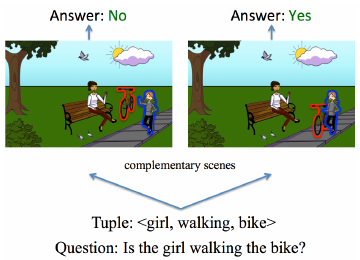
\includegraphics[width=0.35\textwidth]{zhang2016yin_balancing_procedure.png}
    \caption{\citeauthor{zhang2016yin} demonstrate their answer distribution balancing technique. Given the scene on the left and the question ``Is the girl walking the bike'', workers were tasked with creating a scene that differs from the scene on the left but has the opposite answer to the question, as illustrated by the scene and answer on the right.}
    \label{fig:zhang2016yin_balancing_procedure}
\end{figure}

Despite this method's success in reducing the proportion of unbalanced (image, question) pairs by almost 72\%, 20.48\% (image, question) pairs in the balanced dataset did not have a complementary (image, question) pair; 5.93\% because a complementary scene could not be created due to limitations of the abstract scenes clip-art library, and 14.55\% due to disagreement between the answers collected by workers for a given scene. A similar approach was used for non-binary questions in the creation of the VQA 2.0 dataset, as summarised in Table \ref{tab:dataset_comparison} above. \citeauthor{hudson2019gqa} approach the task of dataset balancing from a different angle, aiming to mitigate biases in the answer distributions of the GQA dataset whilst maintaining some degree of representation of real-world priors.

Whilst it is certainly important that dataset creators mitigate biases in their work, it is also the responsibility of VQA model authors to ensure that the ways in which image and question data is fed to their models is also able to be justified; many models,  incorporate BiLSTMs \cite{hudson2018compositional} or LSTMs \cite{andreas2016neural} to obtain question-level representations, however by processing the input data in this manner, it becomes difficult to determine the extent to which the reasoning part of the model is exploiting probabilistic priors in the dataset. By embedding and processing the question as a graph, interpretability studies can be performed on the model to ensure the reasoning part of the model performs as intended.

\section{Visual Question Answering Methods}
\label{section:vqa_methods}

It has been observed that the architectures that leverage additional information such as scene graphs rather than just raw image features tend to perform better. This is clearly illustrated by \citeauthor{hudson2019gqa_preprint} in Figure \ref{fig:gqa_input_representation} below:

\begin{figure}[H]
    \centering
    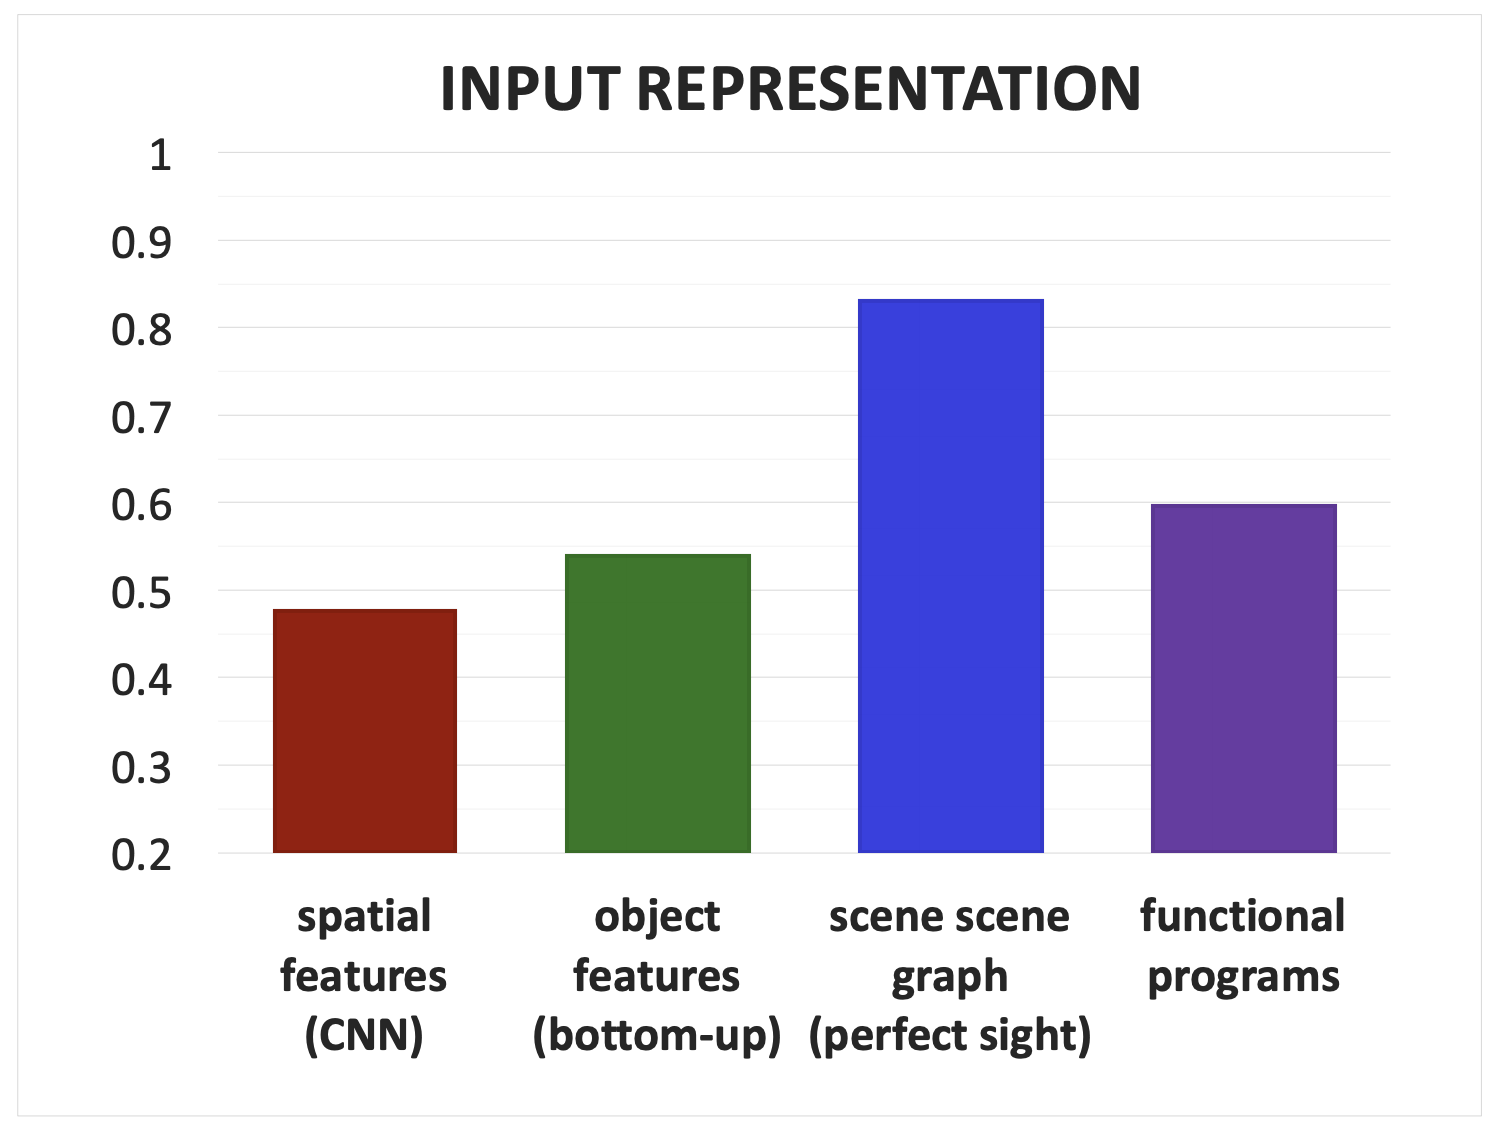
\includegraphics[width=0.5\textwidth]{gqa_input_representation.png}
    \caption{\citeauthor{hudson2019gqa_preprint} illustrate the effect of various forms of input embeddings, noting that accuracy of the trained MAC network \cite{hudson2018compositional} increases drastically with the semantic richness of the embedding.}
    \label{fig:gqa_input_representation}
\end{figure}

\citeauthor{hudson2018compositional} rightly point out that scene graphs cannot always be relied on as a supervisory data source, however with the rise of new scene graph generation models, scene graphs can be generated automatically from images. Since these graphs no longer have to be created through labour-intensive means as seen in the Visual Genome dataset, the use of scene graphs as an image embedding is more feasible, as they can be created quickly for any input image.

\vspace{\baselineskip}

Despite this, very few (if any) models are effectively using similar graph embeddings for question data. By embedding this data similarly to the image, it becomes possible to perform reasoning steps about the image based on the question and vice versa. Commonly used image and quesion embeddings include:

\subsubsection*{Image Representations}
\addcontentsline{toc}{subsubsection}{Image Representations}

\begin{itemize}
    \item CNN features
    \item Image object features and annotations
    \item Scene Graphs
\end{itemize}

\subsubsection*{Question Representations}
\addcontentsline{toc}{subsubsection}{Question Representations}

\begin{itemize}
    \item Traditional word embeddings e.g. word2vec, GloVe
    \item Recurrent neural network embeddings, e.g. LSTM, GRU and their bidirectional counterparts. 
    \item Dependency-based word embeddings \cite{levy2014dependency}
    \item Functional Programs
\end{itemize}

\subsubsection*{Combined Question and Image Representations}
\addcontentsline{toc}{subsubsection}{Combined Question and Image Representations}

\begin{itemize}
    \item Question-Image co-attention \cite{lu2016hierarchical}
    \item Bilinear models e.g. BLOCK Fusion \cite{ben2019block}
\end{itemize}


\subsubsection*{Module Networks}
\addcontentsline{toc}{subsubsection}{Module Networks}

Whilst deep neural networks have proved useful for many classification tasks due to their inherent ability to extract correlations between input and output, they are difficult to interpret and struggle to perform complex reasoning tasks. In order to increase interpretability and coerce deep learning models to perform more structured reasoning steps, \citeauthor{andreas2016neural} proposed the creation of multiple network `modules', each capable of performing a specific reasoning step, similar to each component of the functional programs found in the CLEVR \cite{johnson2017clevr} and GQA \cite{hudson2019gqa} datasets.

\vspace{\baselineskip}

Whilst attaining a state-of-the-art result in 2016 on the VQA 1.0 test dataset \cite{antol2015vqa} of 58.7\%, the per-question-type statistics report only a 2.5\% and 1.4\% performance improvement over a LSTM language-only baseline on binary and numerical questions despite the 16\% improvement on `other'-type questions. This suggests that the success of the model is likely clouded by statistical biases in the dataset, evidenced by the use of a text-only model in the ensemble shown in Figure \ref{fig:andreas2016neural_neural_module_network}. As discussed by \citeauthor{hudson2018compositional}, the model depends on unreliable parsers and their ``hand-crafted'' design lacks extensibility. Moreover, attention maps on raw CNN features are used as the primary form of image data input. Whilst supplementary information like scene graphs and object annotations were not available at the time of writing, these data formats would allow for additional interactions and data transfer between modules, likely improving the network's ability to perform logical reasoning processes.

\begin{figure}[H]
    \centering
    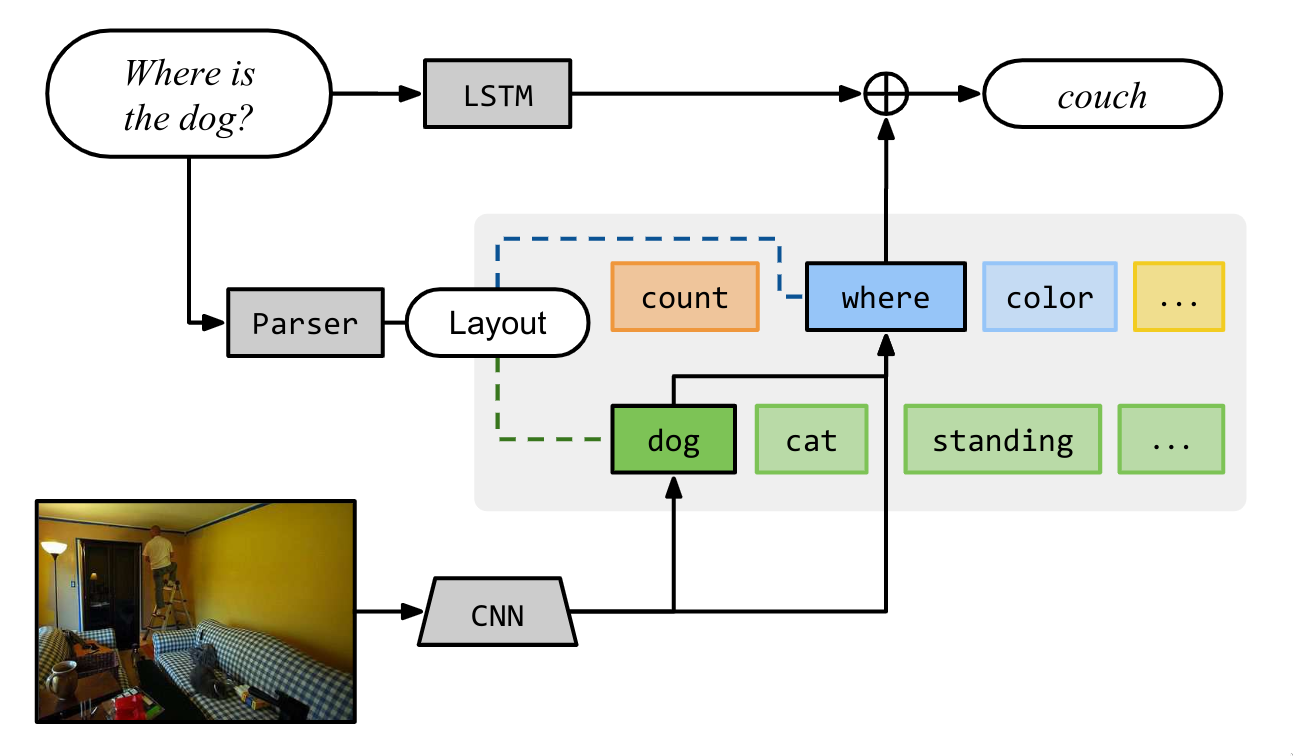
\includegraphics[width=0.5\textwidth]{module_network.png}
    \caption{\citeauthor{andreas2016neural} propose the Neural Module Network, in which reasoning operations are strung together based on parser outputs and use combinations and transformations of attention maps on image features to predict a final answer to the question.}
    \label{fig:andreas2016neural_neural_module_network}
\end{figure}

\citeauthor{andreas2016learning} improve upon their earlier work with a more robust method for generating compositional module layouts from questions, combining LSTM embeddings of the question with representations of candidate module layouts to select a module layout using a reinforcement learning approach. This model sees only a slight improvement over their previous iteration, however provides a novel framework for a variety of graph-based reasoning tasks; the scene graphs and functional programs in CLEVR and GQA are strong supervisory training data for such models, and recent scene graph generation techniques \cite{yang2018graph} would prove useful in generalising models to images that have not been previously annotated.

% \subsubsection*{Attention Mechanisms}
% \addcontentsline{toc}{subsubsection}{Attention Mechanisms}

% Attention mechanisms have gained traction in the research community recently, with the rise of non-recurrent models like the Transformer \cite{vaswani2017attention}, and pre-trained models like BERT \cite{devlin2018bert}. Many have realised their potential for multi-modal reasoning tasks, using a variety of attention-based mechanisms to aid reasoning processes.

% \vspace{\baselineskip}

% \citeauthor{hudson2018compositional} leverage the power of self-attention in their Memory-Attention-Composition cell, heavily inspired by recurrent architectures like LSTMs and GRUs. Aiming to shift the focus of VQA models from 
% Bottom-Up and Top-Down:

% MAC: Good, interpretable, but uses BiLSTM for embedding and raw spatial features. What about scene graphs and dependency-based embeddings? (BLOCK-MAC)

% DMCN: 

% DFAF:

% DCAF:

% Hierarchical Question-Image Co-Attention for Visual Question Answering

% - BLOCK:
%   - More efficient than simple bilinear models
%   - Fewer trainable parameters than other fusion techniques, yet outperforms six novel fusion methods.
%   - Not interpretable
  
% - MAC:
%   - Interpretable
%   - Does not use scene graphs or functional programs for supervision, however show a drastic improvement

% \subsubsection*{Multi-Modal Fusion}
% \addcontentsline{toc}{subsubsection}{Multi-Modal Fusion}

% BLOCK Superdiagonal Fusion: Performs decently in terms of VQA metrics, and performs much better than raw bilinear models, however is not interpretable.

% BAN: TODO

\section{Question Embedding in Visual Question Answering}

\section{Image Embedding in Visual Question Answering}

\section{Multi-modal Fusion in Visual Question Answering}


% Model list 8-12

% Focus
% MAC
% Dual channel GCNs
% ReGAT
% Neural state machine

% Others
% Text GCN

% Methodology
% Graph R-CNN
